%
% $RCSfile: transient.tex,v $
%
% Copyright (C) 2002-2008. Christian Heller.
%
% Permission is granted to copy, distribute and/or modify this document
% under the terms of the GNU Free Documentation License, Version 1.1 or
% any later version published by the Free Software Foundation; with no
% Invariant Sections, with no Front-Cover Texts and with no Back-Cover
% Texts. A copy of the license is included in the section entitled
% "GNU Free Documentation License".
%
% http://www.cybop.net
% - Cybernetics Oriented Programming -
%
% http://www.resmedicinae.org
% - Information in Medicine -
%
% Version: $Revision: 1.1 $ $Date: 2008-08-19 20:41:09 $ $Author: christian $
% Authors: Christian Heller <christian.heller@tuxtax.de>
%

\subsubsection{Transient}
\label{transient_heading}
\index{Transient Communication}
\index{Direct Communication}
\index{Assembler}
\index{Mapper}
\index{Translator}
\index{Signal Processing}

Valentin Turchin \cite{turchin} writes:

\begin{quote}
    Sensations are produced by our sense organs. Perceptions are formed and used
    within the brain. Conceptions are created by ourselves while we create new,
    linguistic, models of the world.
    The triad: Sensation, Perception, Conception seems close in meaning to Kant's
    usage of these terms. We leave it to the reader, though, to judge on it.
\end{quote}

The following example demonstrates a typical information processing procedure.
Its sequential flow is illustrated in figure \ref{handling_figure} which uses
technical names, instead of biological ones. These can be found again in the
explaining text, enclosed in parentheses. The terms \emph{Assembler} and
\emph{Mapper} are converted and merged into the term \emph{Translator}.

\begin{figure}[ht]
    \begin{center}
        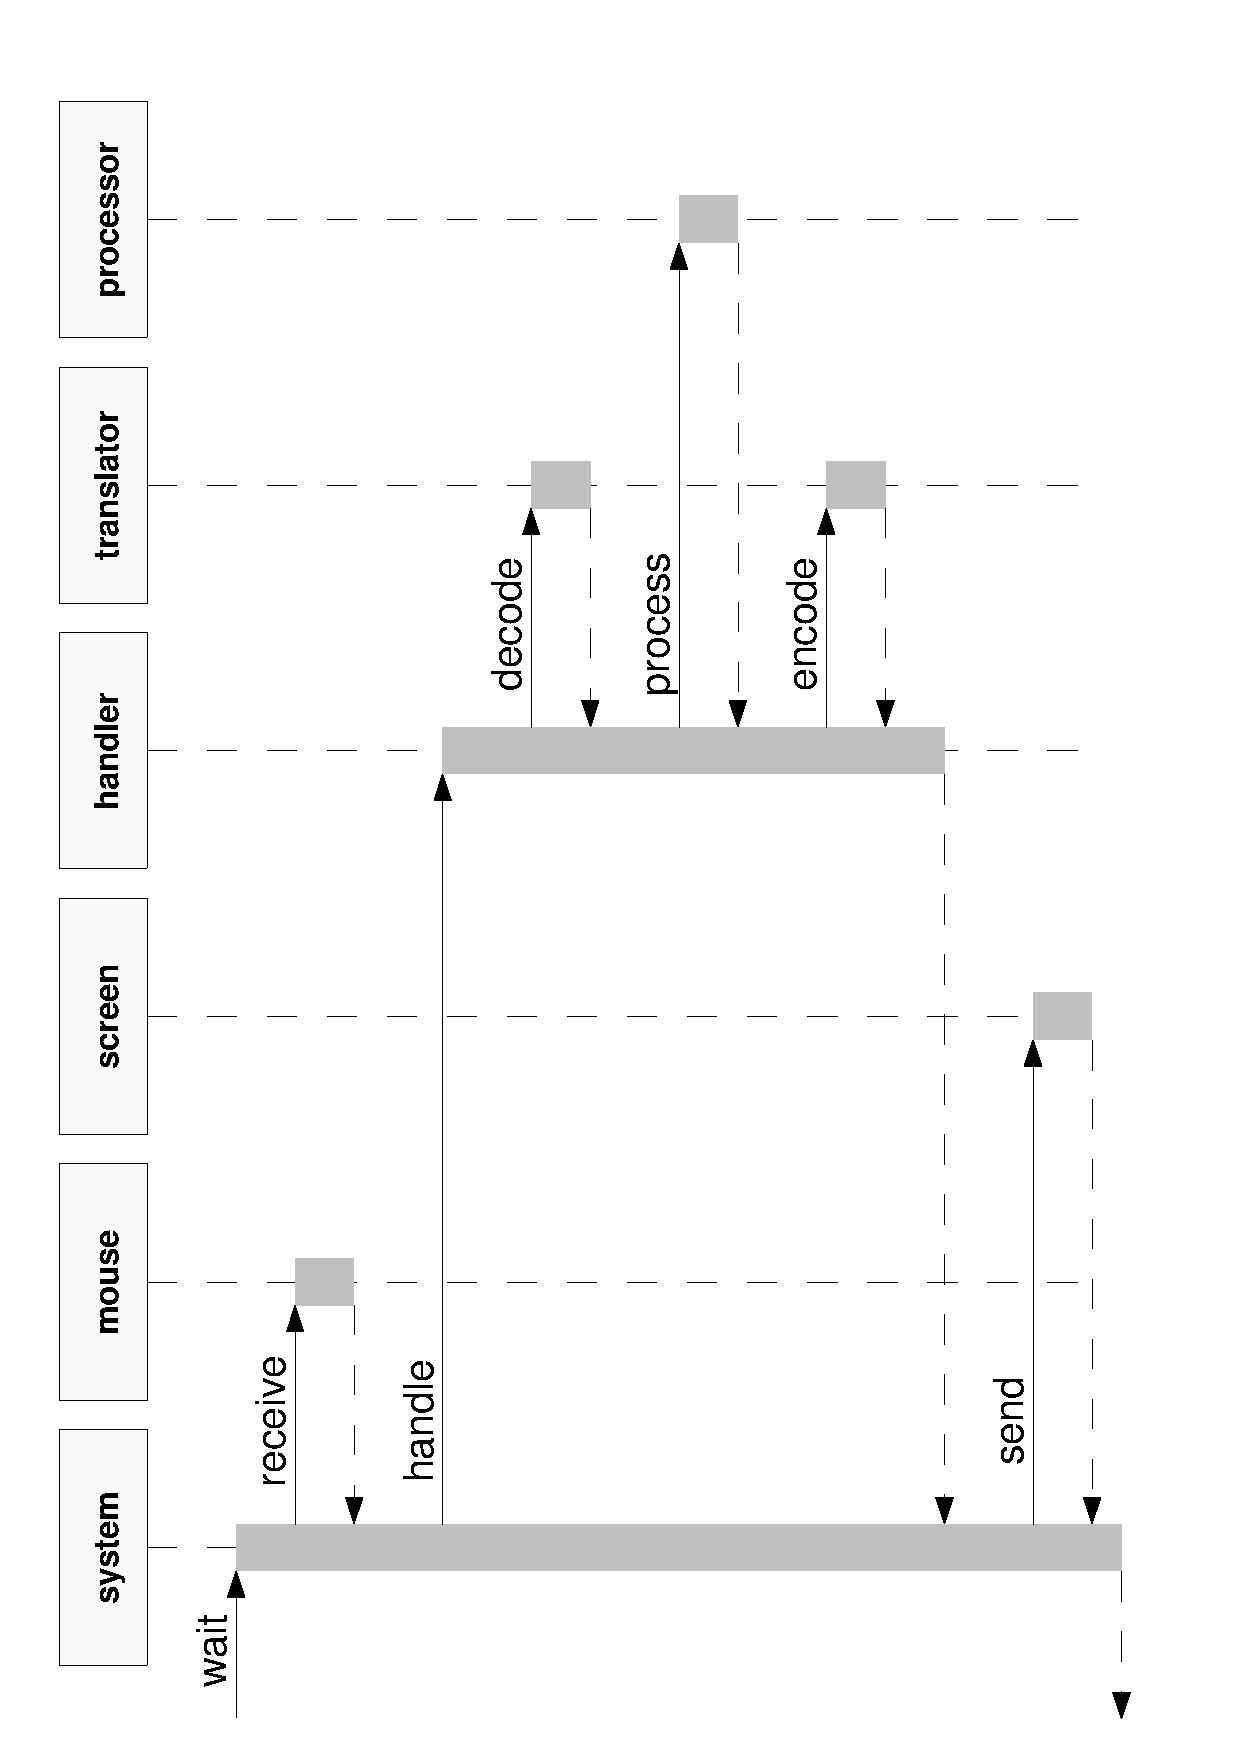
\includegraphics[scale=0.3,angle=-90]{graphic/handling.pdf}
        \caption{Signal Processing as UML Sequence Diagram}
        \label{handling_figure}
    \end{center}
\end{figure}

One human being (\emph{System}) wants to send a message to another. It decides
for an acoustical message (\emph{Signal}), formulates a sentence and talks. The
other human being, waiting for signals (\emph{wait}), receives the message
across its ear organ (\emph{Microphone}, \emph{Keyboard}, \emph{Mouse}). The
message is then forwarded to the receiver's brain (\emph{Handler}), where a
special region responsible for acoustics (\emph{Translator}) translates
(\emph{decode}) the data (\emph{Data Transfer Model}) contained in the message
and sorts them into the human's abstract model of the surrounding real world
(\emph{Domain Model}). Processing of the message happens in the cerebral cortex
of the brain (\emph{Processor}). If the addressed listener wants to send an
answer message (\emph{Signal}), it may do so by triggering a muscle reaction.
For this to happen, the motoric brain region (\emph{Translator}) needs to
translate (\emph{encode}) model data (\emph{Domain Model}) into a special
transfer model (\emph{User Interface Model}), for the answer. Finally, the
answer message (\emph{Signal}) will be sent as muscle action (data display on
\emph{Monitor}).

If a communication partner does not, or only partly receives a message, the
missing information is lost, unless the sender repeats it once more. The reason
is that the transport mediums (light, air) do not steadily contain the
information; the sent information is transient. Therefore, the whole process
described above can be called \emph{Transient Communication}.
